\documentclass[11pt]{article}
\usepackage{graphicx}
\usepackage{float}
\usepackage{hyperref}
\usepackage{natbib}
\usepackage{listings}
\usepackage{xcolor}
\usepackage[dvipsnames]{xcolor}
\usepackage[svgnames]{xcolor}
\usepackage{amsmath} % For the equation* environment
\usepackage{amssymb}

\hypersetup{
    colorlinks=true,
    linkcolor=red,
    filecolor=cyan,      
    urlcolor=orange,
    pdftitle={Overleaf Example},
    pdfpagemode=FullScreen,
    }

\setlength{\textwidth}{6.5in}
\setlength{\headheight}{0in}
\setlength{\textheight}{8.0in}
\setlength{\hoffset}{0in}
\setlength{\voffset}{0in}
\setlength{\oddsidemargin}{0in}
\setlength{\evensidemargin}{0in}

\lstdefinestyle{txtstyle}{
    basicstyle=\ttfamily\small,
    breaklines=true,
    backgroundcolor=\color{Bisque}
}
\lstset{style = txtstyle}

\definecolor{codegreen}{rgb}{0,0.6,0}
\definecolor{codegray}{rgb}{0.5,0.5,0.5}
\definecolor{codepurple}{rgb}{0.58,0,0.82}
\definecolor{backcolour}{rgb}{0.95,0.95,0.92}

\lstdefinestyle{mystyle}{
    backgroundcolor=\color{backcolour},   
    commentstyle=\color{codegreen},
    keywordstyle=\color{magenta},
    numberstyle=\tiny\color{codegray},
    stringstyle=\color{codepurple},
    basicstyle=\ttfamily\footnotesize,
    breakatwhitespace=false,         
    breaklines=true,                 
    captionpos=b,                    
    keepspaces=true,                                   
    numbersep=5pt,                  
    showspaces=false,                
    showstringspaces=false,
    showtabs=false,                  
    tabsize=2
}

\title{Computational Physics ps-9 Report}
  
\author{Tongzhou Wang, \\ GitHub account: TZW56203, repository: phys-ga2000. \\ \url{https://github.com/TZW56203/phys-ga2000}}

\date{November 24, 2024}

\begin{document}

\maketitle

\section{Problem 1}

\subsection{Part (a) and (b)}
The second-order differential equation
\begin{equation}
    \frac{d^2 x}{dt^2} = -\omega^2 x.
\end{equation}
can be put into two first-order differential equations
\begin{equation}
    \begin{cases}
        \frac{dx}{dt} = y, \\
        \frac{dy}{dt} = -\omega^2 x.
    \end{cases}
\end{equation}

Figure \ref{fig:harmonic} shows the motion of a harmonic oscillator. We can observe that as we increase the amplitude by making the initial value of $x$ bigger, the period stays roughly the same.
\begin{figure}[H]
    \centering
    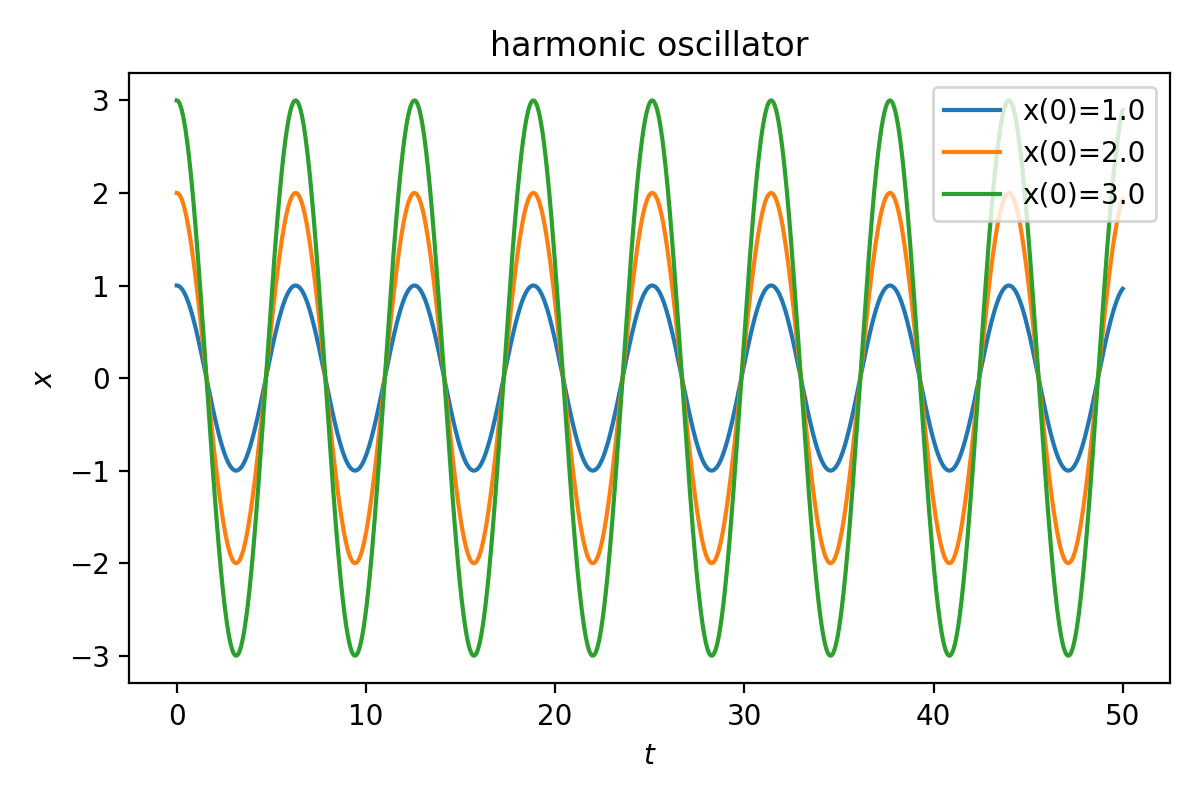
\includegraphics[scale = 0.7]{Figs/ps-9-1ab.png}
    \caption{Harmonic oscillator.}
    \label{fig:harmonic}
\end{figure}

\subsection{Part (c) and (d)}
Figure \ref{fig:anharmonic} shows the motion of an anharmonic oscillator. We can observe that the larger the amplitude, the shorter the period, that is, the faster the oscillation.
\begin{figure}[H]
    \centering
    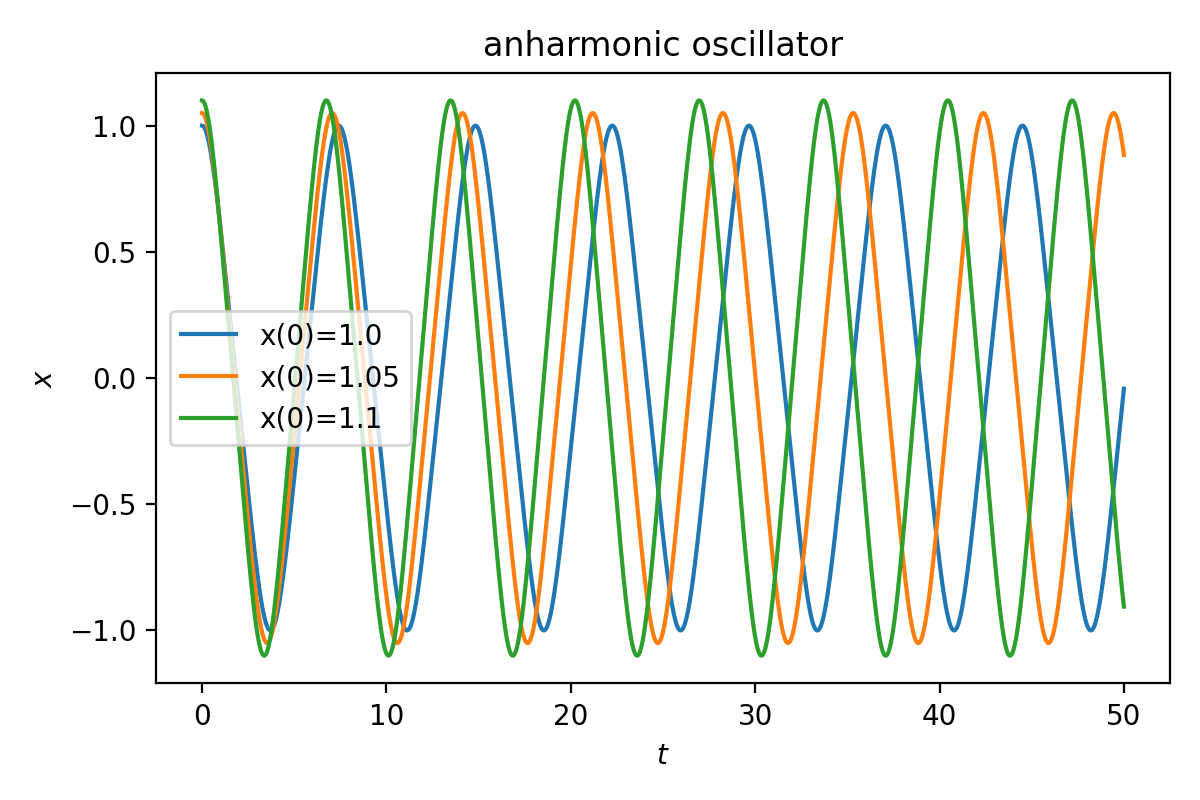
\includegraphics[scale = 0.7]{Figs/ps-9-1c.png}
    \caption{Anharmonic oscillator.}
    \label{fig:anharmonic}
\end{figure}

Figure \ref{fig:anharmonic-ps} shows the phase space diagram of the anharmonic oscillator.
\begin{figure}[H]
    \centering
    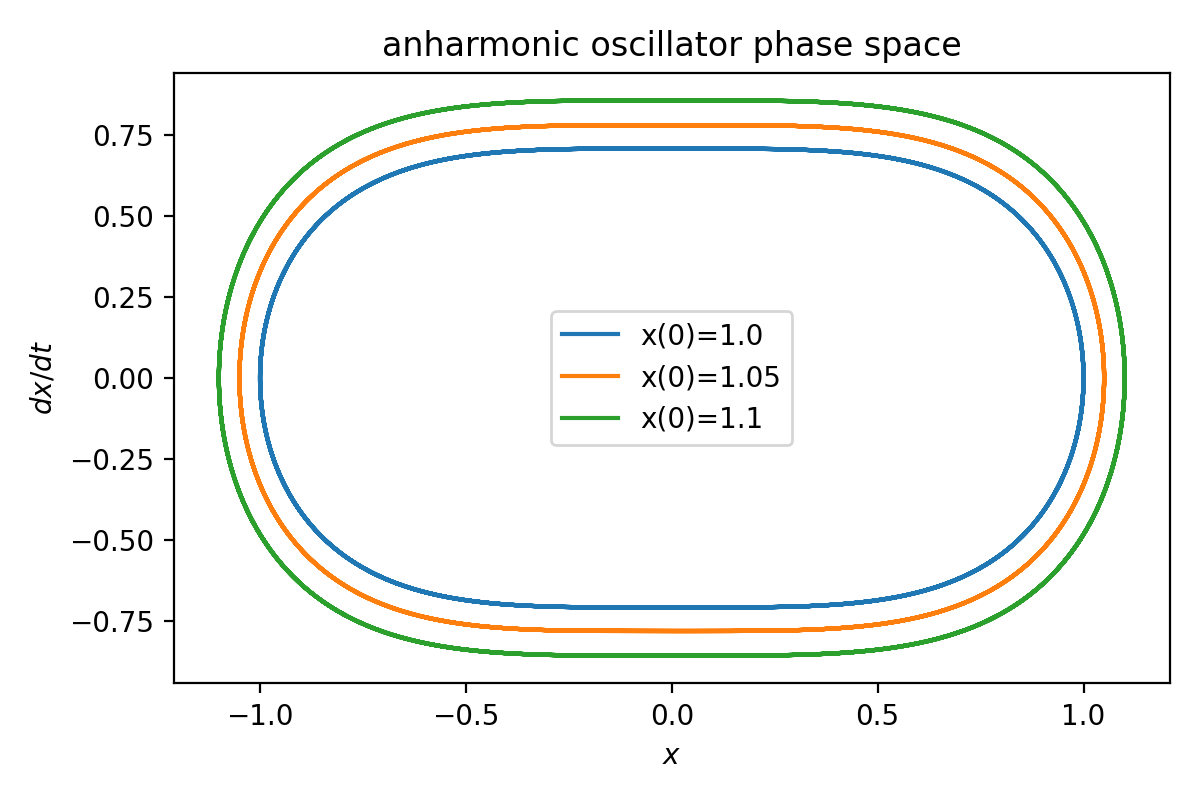
\includegraphics[scale = 0.7]{Figs/ps-9-1d.png}
    \caption{Anharmonic oscillator phase space.}
    \label{fig:anharmonic-ps}
\end{figure}

\subsection{Part (e)}
Figure \ref{fig:vdp} shows the phase space diagram of the van der Pol oscillator.
\begin{figure}[H]
    \centering
    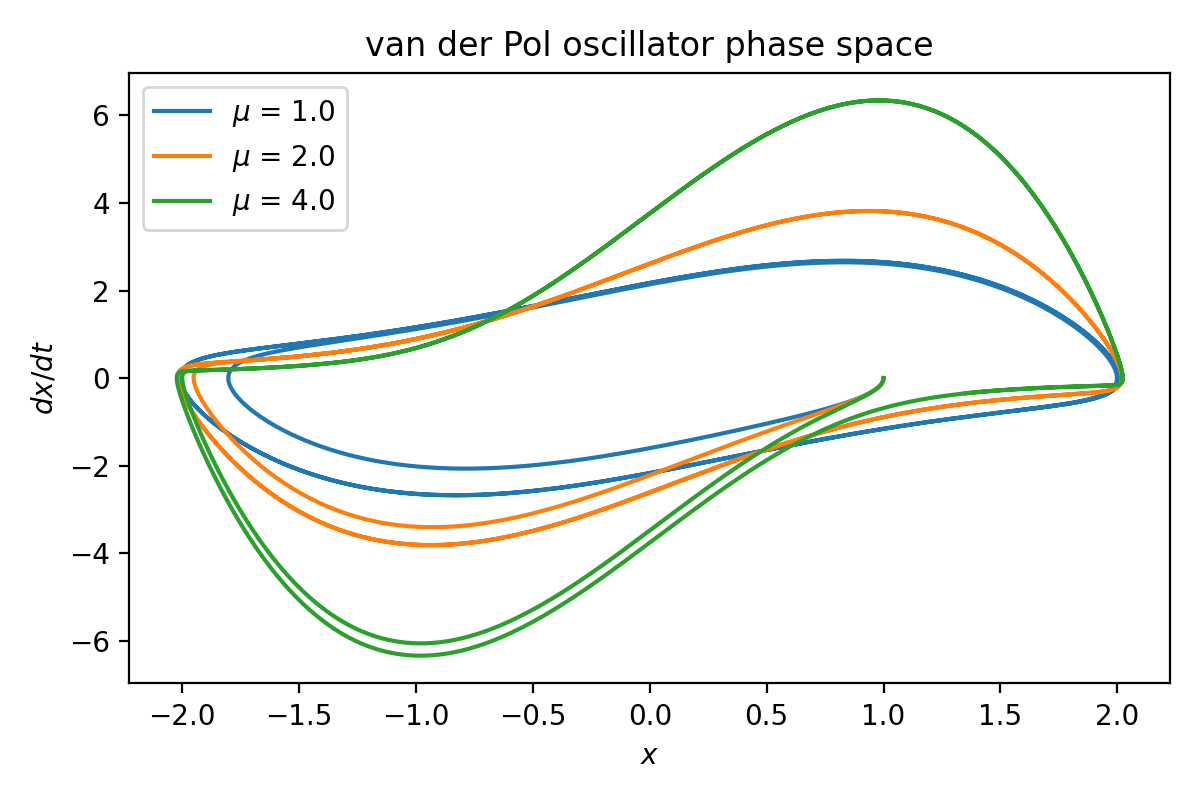
\includegraphics[scale = 0.7]{Figs/ps-9-1e.png}
    \caption{van der Pol oscillator phase space.}
    \label{fig:vdp}
\end{figure}

\section{Problem 2}

\subsection{Part (a)}
The Newton's second law gives
\begin{equation}
\begin{gathered}
    -\frac{1}{2}\pi R^2 \rho C (\dot{x}^2 + \dot{y}^2) \frac{\dot{x}}{\sqrt{\dot{x}^2 + \dot{y}^2}} = m \ddot{x}, \\
    -mg -\frac{1}{2}\pi R^2 \rho C (\dot{x}^2 + \dot{y}^2) \frac{\dot{y}}{\sqrt{\dot{x}^2 + \dot{y}^2}} = m \ddot{y}.
\end{gathered}
\end{equation}
Rearranging, we get
\begin{equation}
\begin{gathered}
    \ddot{x} = -\frac{\pi R^2 \rho C}{2m} \dot{x} \sqrt{\dot{x}^2 + \dot{y}^2}, \\
    \ddot{y} = -g -\frac{\pi R^2 \rho C}{2m} \dot{y} \sqrt{\dot{x}^2 + \dot{y}^2}.
\end{gathered}
\end{equation}

We can take 
\begin{equation}
    t^\prime = \frac{t}{T}, \ x^\prime = \frac{x}{gT^2}, \ y^\prime = \frac{y}{gT^2}.
\end{equation}
For convenience, we define
\begin{equation}
\begin{gathered}
    \frac{R^2 \rho C g T^2}{m} \equiv k, \\
    \frac{dx^\prime}{dt^\prime} \equiv v_x, \\
    \frac{dy^\prime}{dt^\prime} \equiv v_y.
\end{gathered}
\end{equation}
Thus, the equations are rescaled to become
\begin{equation}
\begin{gathered}
    \frac{dv_x}{dt^\prime} = -\frac{\pi}{2} k v_x \sqrt{v_x^2 + v_y^2}, \\
    \frac{dv_y}{dt^\prime} = -1 - \frac{\pi}{2} k v_y \sqrt{v_x^2 + v_y^2}.
\end{gathered}
\end{equation}

\subsection{Part (b) and (c)}
Figure \ref{fig:y-x} and \ref{fig:yp-xp} show the trajectories of the cannonball in the rescaled and original variables respectively. We can observe that the heavier the cannonball (the smaller the value of $k$), the further it travels.
\begin{figure}[H]
    \centering
    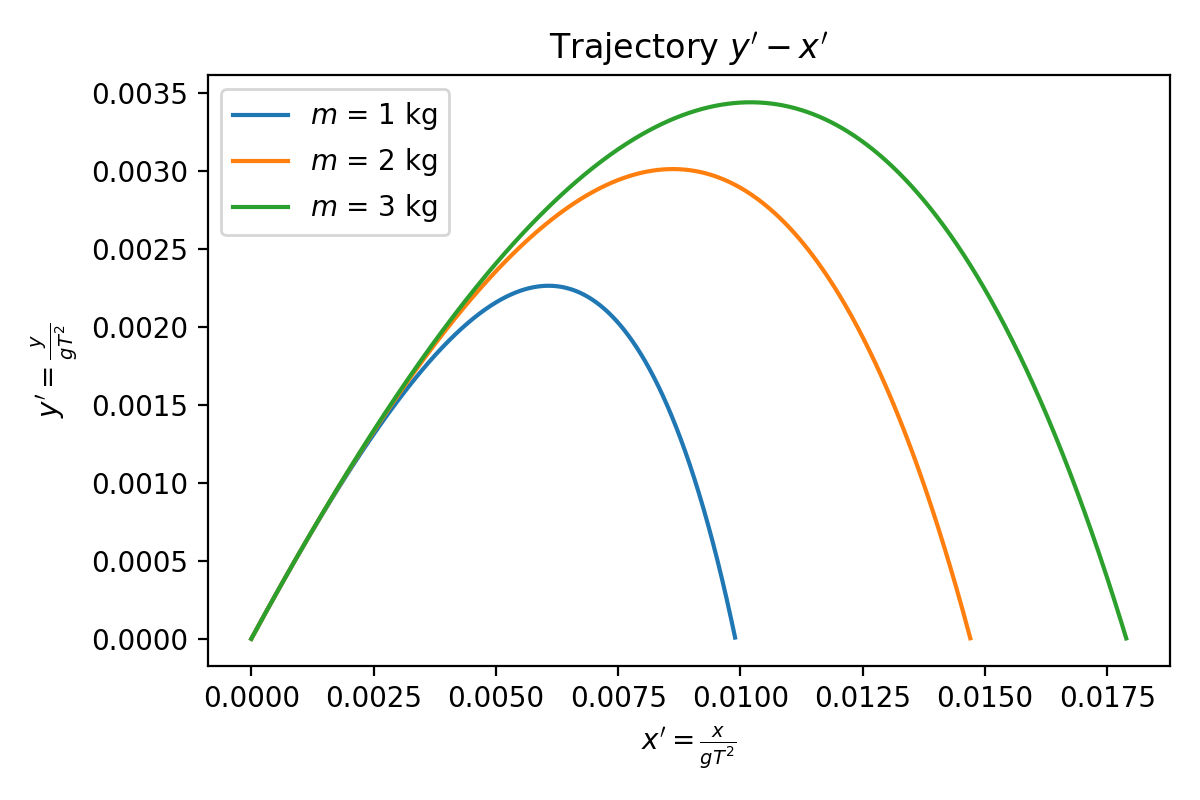
\includegraphics[scale = 0.7]{Figs/ps-9-2.png}
    \caption{Trajectory in rescaled variables.}
    \label{fig:y-x}
\end{figure}
\begin{figure}[H]
    \centering
    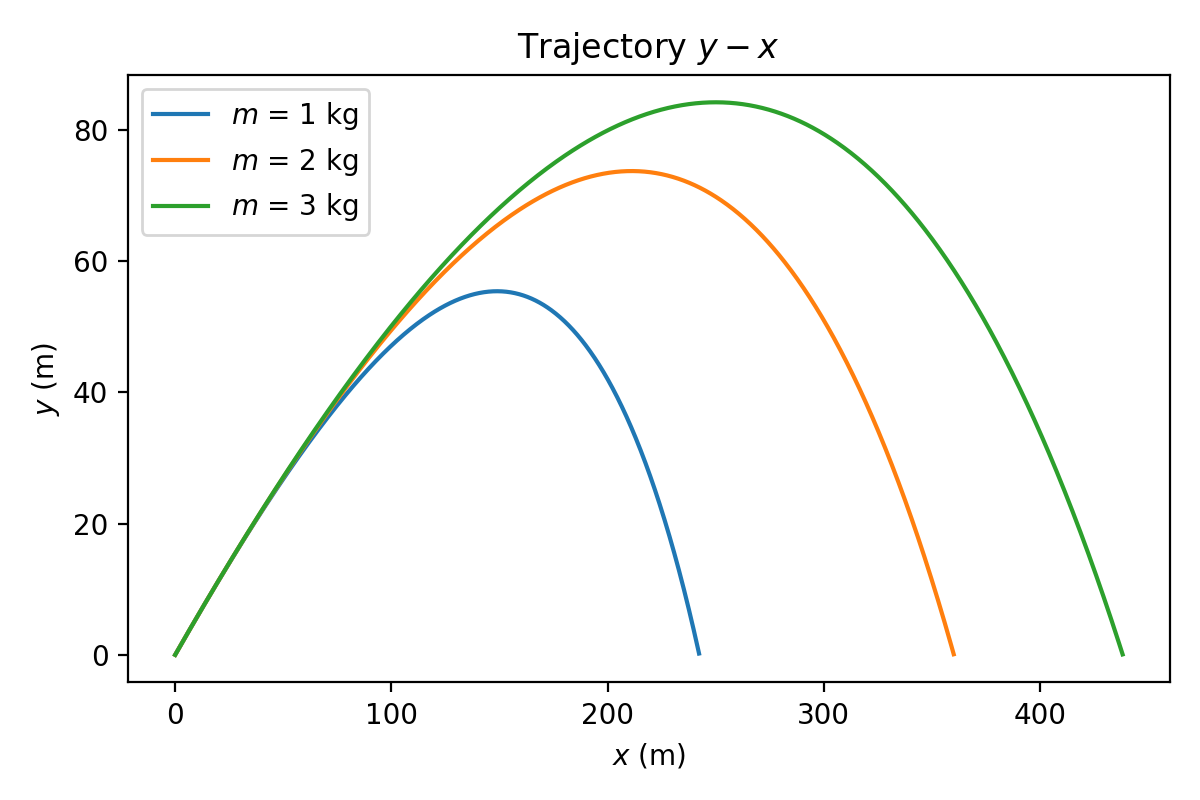
\includegraphics[scale = 0.7]{Figs/ps-9-2unit.png}
    \caption{Trajectory in original variables.}
    \label{fig:yp-xp}
\end{figure}

\end{document}
